%\documentclass[a4paper,landscape,twocolumn,12pt]{article}
\documentclass[a4paper,12pt]{article}

\usepackage[french]{babel}
\usepackage[utf8]{inputenc}
\usepackage[T1]{fontenc}
\usepackage{graphicx}
\usepackage{tabularx}
\usepackage{color}
\usepackage{tikz}\usetikzlibrary{shapes.geometric}
\usepackage{url}
\usepackage{import,palatino}
\usepackage{pdfpages,wrapfig,setspace}
\usepackage[margin=15mm]{geometry}

\setlength{\parskip}{\smallskipamount}
%\setlength{\parindent}{0pt}

\pagestyle{empty}
\begin{document}
\begin{center}
  {\Huge Ceci est un petit livre}

  {\Large à construire vous-même}
\end{center}

\large

Vous trouverez de ce côté les instructions de fabrication de votre
petit livre, qui se trouve de l'autre côté de la feuille. Pas besoin
de colle, uniquement des ciseaux :

\bigskip\bigskip

\noindent\textbf{À l'impression}, assurez-vous que le document n'est
pas remis à l'échelle. Si votre logiciel vous donne le choix, demandez
à imprimer à 100\%, sans redimensionner.

\medskip
\noindent\textbf{Étape 1 :} Pliez votre feuille en deux.
Les bords doivent être bien jointifs.

\noindent
\begin{minipage}[b]{.45\linewidth}
\medskip
\noindent\textbf{Étape 2 :} Repliez encore en deux, puis encore en deux. Les plis doivent être
bien marqués.

\medskip \centerline{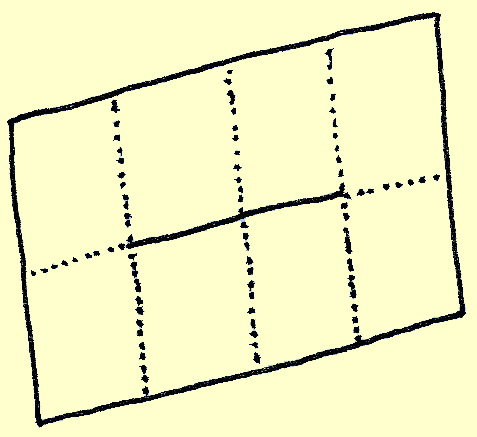
\includegraphics{img/ptitlivre-etape2.jpg}}

\medskip
\noindent\textbf{Étape 4 :} Repliez la feuille dans le sens de la longueur.\\

  \centerline{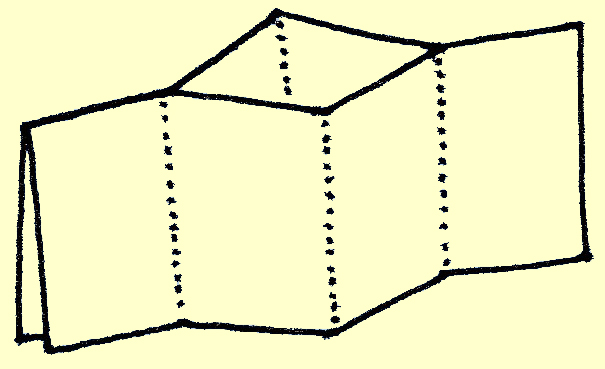
\includegraphics{img/ptitlivre-etape4.jpg}}

\end{minipage}\hfill\begin{minipage}[b]{.45\linewidth}
\noindent\textbf{Étape 3 :} Découpez le pli au milieu de la page.

\bigskip
\bigskip \centerline{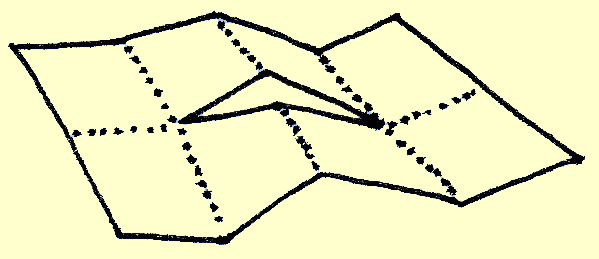
\includegraphics{img/ptitlivre-etape3.jpg}}
  
\bigskip
\bigskip
\bigskip
\bigskip
\noindent\textbf{Étape 5 :} Repliez les deux parties centrales, repliez
le tout et c'est fini !

  \centerline{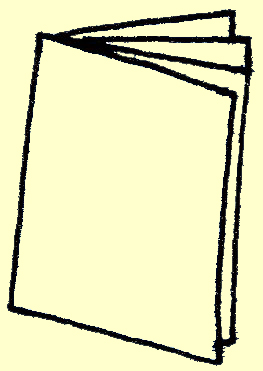
\includegraphics{img/ptitlivre-etape5.jpg}}

\bigskip
\end{minipage}

\bigskip~\hfill{\small Le concept du «~petit livre~» est une idée
  originale de {\color{blue}\url{http://petitslivres.free.fr/}}}

\bigskip \bigskip \bigskip %
Ce petit livre, créé par Martin Quinson et Jean-Christophe Bach, est
diffusé en CC-BY-SA. Merci de nous indiquer toute erreur ou
amélioration possible sur :

\centerline{\color{blue}\url{https://github.com/jcb/CSIRL}}

\bigskip%
Il s'agit de la version du 6 février 2014.
\end{document}
